\section{Force estimation}
%%%%%%%%%%%% MID WAY AGENDA %%%%%%%%%%%%%%
\begin{frame}<beamer>
\frametitle{Filip Maric}
\tableofcontents[currentsection]
\end{frame}


% the license
\begin{frame}{Force estimation model}{}

%\begin{columns}[T]
%\begin{column}{\textwidth}

  \begin{itemize}
    \item<1-> Model approach
    \item Nonlinearities in the EndoWrist dynamics    
    \begin{itemize}
      \item Hammerstein Wiener Models
    \end{itemize}
  \end{itemize}
%\end{column}%
%\hfill%
%\begin{column}{.65\textwidth}

\vspace{3em}
\begin{figure}[H]
\resizebox{0.9\textwidth}{!}{
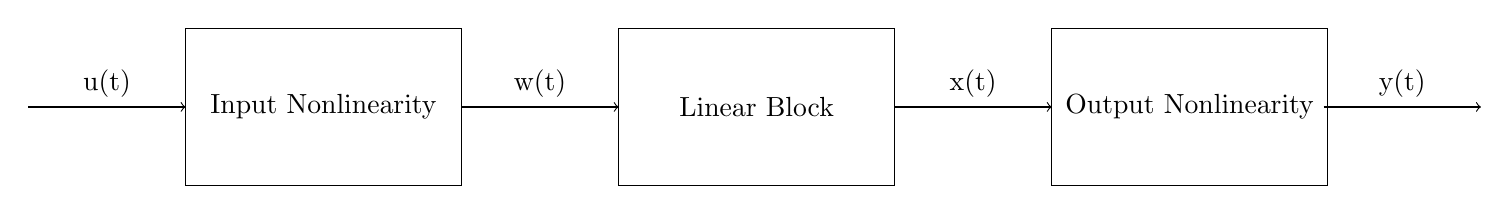
\begin{tikzpicture}
\draw  (-3.5,3) rectangle (0,1) node[pos=.5] {Linear Block};
\draw  (-9,3) rectangle (-5.5,1) node[pos=.5] {Input Nonlinearity};
\draw  (2,3) rectangle (5.5,1) node[pos=.5] {Output Nonlinearity};
\draw [->] (-5.5,2) -- (-3.5,2) node [pos=0.5,above] {w(t)};
\draw [->] (-11,2) -- (-9,2) node [pos=0.5,above] {u(t)};
\draw [->] (0,2) -- (2,2) node [pos=0.5,above] {x(t)};
\draw [->] (5.45,2) -- (7.45,2) node [pos=0.5,above] {y(t)};
\end{tikzpicture}
}
\caption{Hammerstein-Wiener model.}
\label{weiner}
\end{figure}


%\end{column}
%\end{columns}

\end{frame}



%%%%%%%%%%%%%%%%%%%%%%%%%%%%%%%%%%%%%%%%%%%%%%%%%%%%%%%%%%%%%%%%%%%%%%%%%%%%%%%%%%%

\begin{frame}{Force estimation model}{Linear model}
\begin{itemize}
\item Linear model
  \begin{itemize}
  \item Choice of inputs affects model quality
  \item Inputs: effort, velocity 
  \item Outputs: force
  \end{itemize}
\item Black-box identification
	\begin{itemize}
	\item Subspace identification
	\item Hankel singular value analysis
	\end{itemize}
\end{itemize}

Include picture with effort force fit here!! 
% Include effort force picture 
% \begin{figure}[H]
% \centering
% \includegraphics[width=1\textwidth]{hankel}
% \caption{Comparison of Hankel sigular values for different system orders.}
% \label{hankel}
% \end{figure}


\end{frame}

%%%%%%%%%%


\begin{frame}{Force estimation model}{Hammerstein Wiener Models}
\begin{itemize}
\item Input and output nonlinearities
  \begin{itemize}
  \item Effort 
  \item Force
  \end{itemize}
\end{itemize}

Include picture with effort force fit here!! 

% Include effort force picture 
% \begin{figure}[H]
% \centering
% \includegraphics[width=1\textwidth]{hankel}
% \caption{Comparison of Hankel sigular values for different system orders.}
% \label{hankel}
% \end{figure}


\end{frame}




%%%%%%%%%%%%%%%%%%%%%%%%%%%%%%%%%%%%%%%%%%%%%%%%%%%%%%%%%%%%%%%%%%%%%%%%



\begin{frame}{Force estimation model}{Hammerstein Wiener Models}
\begin{itemize}
  \item Nonlinearities
  \begin{itemize}
    \item Deadzone nonlinearities
    \item Input/Output -saturation 
  \end{itemize}
\end{itemize}




include two pictures here worksheet 4.6, 4.6 or 4.7



\begin{columns}[T]
\centering
\begin{column}{.49\textwidth}

% Include effort force picture 
% \begin{figure}[H]
% \centering
% \includegraphics[width=1\textwidth]{hankel}
% \caption{Comparison of Hankel sigular values for different system orders.}
% \label{hankel}
% \end{figure}

\end{column}%
\hfill%
\begin{column}{.49\textwidth}

% Include effort force picture 
% \begin{figure}[H]
% \centering
% \includegraphics[width=1\textwidth]{hankel}
% \caption{Comparison of Hankel sigular values for different system orders.}
% \label{hankel}
% \end{figure}

\end{column}
\end{columns}



\end{frame}




% Include effort force picture 
% \begin{figure}[H]
% \centering
% \includegraphics[width=1\textwidth]{hankel}
% \caption{Comparison of Hankel sigular values for different system orders.}
% \label{hankel}
% \end{figure}








% \begin{frame}{Konklusion}{}
%   \begin{itemize}
%     \item<1-> Analyse af kran  
%     \item<2-> Modeller er blevet udledt på baggrund af analyse  
%     \item<3-> Parameter estimeringer 
%     \item<4-> Root locus er benyttet under udvikling af regulatorer 
%     \item<5-> Strøm offset kan kompensere for statisk friktion
%     \item<6-> Kaskade kobling  
%   \end{itemize}
% \end{frame}




% \begin{frame}{Demonstration}{Simon}
%   \begin{itemize}
%     \item<1-> Kontrol lab
%   \end{itemize}
% \end{frame}
%%%%%%%%%%%%%%%%